\documentclass[border=6pt]{standalone}
\usepackage{amsmath,amssymb}
\usepackage{pgfplots}
\pgfplotsset{compat=1.17}
\begin{document}
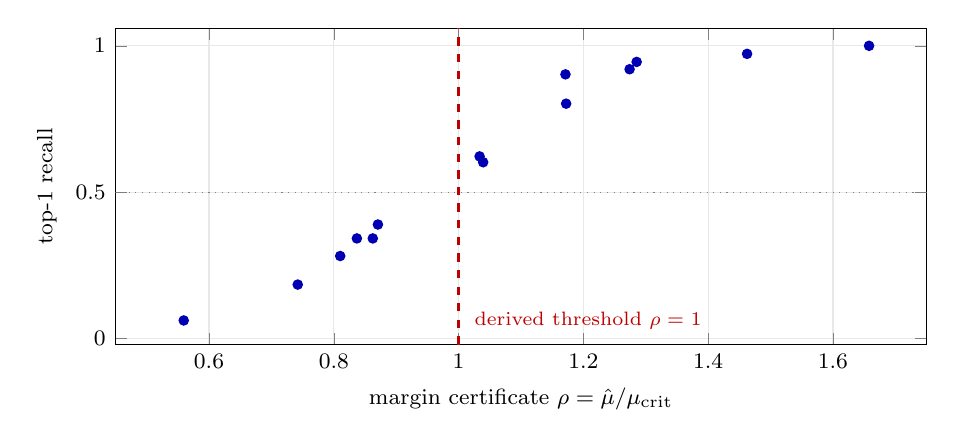
\begin{tikzpicture}
\begin{axis}[
  width=0.98\linewidth, height=5.6cm,
  xlabel={margin certificate $\rho=\hat\mu/\mu_{\mathrm{crit}}$},
  ylabel={top-1 recall},
  xmin=0.45, xmax=1.75, ymin=-0.02, ymax=1.06,
  grid=both, grid style={gray!18},
  tick label style={font=\footnotesize}, label style={font=\footnotesize},
]
\addplot[only marks, mark=*, mark size=1.7pt, blue!70!black] coordinates {
(0.5595,0.0625)(0.7422,0.185)(0.8103,0.2825)(0.837,0.3425)(0.8625,0.3425)
(0.8707,0.39)(1.0337,0.6225)(1.0394,0.6025)(1.1713,0.9025)(1.1724,0.8025)
(1.2741,0.92)(1.2854,0.945)(1.4624,0.9725)(1.6579,1.0)};
\addplot[dashed, red!75!black, thick] coordinates {(1,-0.02)(1,1.06)};
\addplot[dotted, gray] coordinates {(0.45,0.5)(1.75,0.5)};
\node[red!75!black, font=\scriptsize, anchor=south west] at (axis cs:1.01,0.0){derived threshold $\rho=1$};
\end{axis}
\end{tikzpicture}
\end{document}
